%Replace Strings:
%PROJECT.TITLE
%TODO.CHANGE
%PROJECT.ABSTRACT.KEYWORDS

\documentclass[12pt, a4paper, oneside]{article}

\usepackage[utf8]{inputenc}
\usepackage[bindingoffset=1.57cm, left=2.54cm, right=2.54cm, top=2.54cm, bottom=2.54cm]{geometry}
\usepackage{mathptmx}
\usepackage{fancyhdr}
\usepackage{lipsum}
\usepackage{secdot}
\usepackage{lastpage}
\usepackage{cite}

\usepackage{amsmath}
\usepackage{amsfonts}
\usepackage{graphicx}
\usepackage{hyperref}
%\usepackage{tocloft}

\usepackage{caption}

\tolerance=1
\emergencystretch=\maxdimen
\hyphenpenalty=10000
\hbadness=10000



\usepackage{graphicx}
	\graphicspath{ {images/} }

\usepackage{tocloft}
\usepackage[table,xcdraw]{xcolor}

\usepackage{floatrow}
\floatsetup[table]{capposition=bottom}

\linespread{1.2}
\pagestyle{fancy}
\fancyhf{} % sets both header and footer to nothing
\renewcommand{\headrulewidth}{0pt}



%\rhead{ \textit{EcoCycleMart:Ecommerce for Recycled Products}}
\cfoot{\thepage}

\setlength{\parindent}{0pt}
\setlength{\parskip}{12pt}

%\frontmatter

\begin{document}

\pagenumbering{roman}
\addcontentsline{toc}{section}{Abstract}
\large
\begin{center}
	\textbf{ABSTRACT}
\end{center}

\normalsize
Environment is the major source of industrial raw materials. The heavy need of raw materials has been burden for the environment. In the other hand, waste management has been another big issue. This has made us environmentally conscious than ever. We can reduce dependency on environment for raw materials by recycling. For example, Recycling paper reduces the demand for trees to be cut down. Recycling is less energy consuming than manufacturing from scratch. Manufacturing leads to heavy green house gas emissions while the recycling significantly reduces it. Recycling is cost efficient.

EcoCycleMart is the e-commerce platform for the recycled eco-friendly goods where the sellers can list their goods and the buyers can purchase them. The project aims to provide help to the small and medium scale recycling based businesses to find the consumer for their goods. It also ensures consumers, the best quality goods in affordable price. In the long run, the project sets its objective to aware and encourage everyone to use the recycled products for noble cause of environmental protection and sustainability of resources. In summary, this project promotes low capital business, ensures fulfillment of needs for quality products without exploiting environment for resources and minimize the waste management issues.

The major deliverable proposed in the project is a web based application with
user-friendly User Interface and AI based recommendation system .

\textbf{Keywords}: \textit{Environment, Waste, Recycle, E-commerce, EcoCycleMart}\\

\break

\large
\addcontentsline{toc}{section}{Table of Contents}
\begin{center}
	\textbf{TABLE OF CONTENTS}
\end{center}


\normalsize
\setlength{\cftbeforetoctitleskip}{0pt}
\renewcommand{\contentsname}{}
\tableofcontents

\break
%\renewcommand{\cftfigpresnum}{Figure\}
\listoffigures % List of Figures

\break
\listoftables % List of Tables

\break

%\mainmatter
\cfoot{\textbf{\thepage} /  \pageref{LastPage}}

\pagenumbering{arabic}

%INTRODUCTION
\section{Introduction} 
EcoCycleMart is a web based application that provides platform for selling and buying recycled goods. With a view of encouraging the use of recycled goods, the application  aims to fulfill needs for quality goods without exploiting the environment for resources and minimize the waste management issues. In the long term, it targets to conserve environment and maintain ecological balance. This document looks forward to providing essential information about the needs, scope, 
and methodology being used in the application.

E-commerce has a great potential to contribute to the economy and prosperity of nation, but having observation at the statistics, the ratio of contribution of e-commerce is not satisfactory. The recycle based e-commerce market is almost negligible in Nepal. According to Nepal Rastra Bank, the total contribution of the e-commerce to the total GDP of Nepal was almost \$600 million comprising just above than 1\% in 2022/2023.

The government of Nepal has taken efforts to promote recycle based e-commerce. Taking this in consideration the authors are to build the e-commerce web application specially tailored for the low capital recycle based business and consumers looking for goods at affordable price.

The impact on the environment is severe due to the industries . The issues like
climate change, global warming, greenhouse effects etc. has made our planet the ill place to live. In the other hand the waste have been everywhere not managed and left alone. So, why not make use of this thing and contribute towards making earth good place to live.


%PROBLEM STATEMENT
\pagebreak
\subsection{Problem Statement}
In today's consumer-driven society, the massive production and disposal of goods have led to a significant burden on our planet's resources and ecosystems. The linear 'take-make-dispose' model of production and consumption leads to environmental degradation, invites climate change, and accelerates the depletion of finite resources. Despite growing awareness of these issues, there remains a lack of accessible and convenient options for individuals to adopt more sustainable consumption habits.

Furthermore, while recycling is recognized as a crucial component of sustainable waste management, there exists a disconnect between the availability of recycled products and consumer demand. Managing multiple sellers to ensure a diverse and high-quality inventory of recycled goods while maintaining consistent standards and compliance has been pain in neck.
sellers and marketplace administrators need access to detailed analytics and reporting to make informed business decisions. Users want easy access to the curated list of products that suit their need and preference.

\pagebreak
\subsection{Project Objectives}
The project has put forward the following objectives:

\begin{itemize}
	\item To make the alternative solution for ecommerce activities.
		\item{ To use artificial intelligence applications for personalized recommendation.}
		%\item {AI powered product recommendaton.}
	%\item To promote the local, small and Medium enterprises for recyclable products.

	 %\item To aware consumers about the environmental impact of their purchasing choices and the benefits of opting for recycled products.
	 
	%\item User friendly and intuitive website interface to facilitate easy navigation and enhance the shopping experience
	%\item To cater the curated list of products that suit buyers need and %preferences.
%	\item To make the decision making easy and efficient through reporting and analytics.
\item{To use Google Authentication, Payment Integration, Rating and Reviews.}

\end{itemize}

\pagebreak
\subsection{Significance of the Study}
The project is significant owing to the fact that we are living in digital world, and the project will certainly be fruitful in achieving the objectives set by the Government of Nepal regarding Ecological Balance, Waste management and promoting e-commerce. Since the idea is one of the first of its kind, it is expected that the project will reach to a significant majority of sellers and buyers. Understanding the security requirements and compliance regulations helps in implementing robust security measures to protect sensitive data, thereby building trust among users.

Multi-seller marketplaces offer consumers a wide variety of products from different sellers, increasing choices and fostering competitive pricing. By studying the user interface and experience, improvements can be made to provide a seamless, user-friendly shopping experience, enhancing customer satisfaction. Feedback mechanisms ensures that sellers are held to high standards, maintaining the marketplace’s reputation. Implementing AI for catering products based on customer needs, preferences and history.

\pagebreak
\subsection{Scope of the study}
In the beginning phase, the basic e-commerce concept is to be implemented and other features are to be added later gradually if possible. Such possible extensions could be addition of google authentication, AI based recommendation for products, payment integration, rating and reviews etc. The sellers can make their accounts including profiling and list their products in the platform. The buyers can wishlist, add to cart and purchase the products. The users can signin/signup using their google account. They can also rate and review the products. The buyers and sellers both will have separate dashboards. The application able to process payments using the feasible payment providers/services in Nepal.

\pagebreak
\subsection{Limitations of the study}
The following are the limitations of the project that are realized:
\begin{itemize}
 	\item The application is web based but native applications such as mobile and desktop application is not built.
	%\item The application will not be able to ensure the quality and detect if the product being listed is recycled or not .
%	\item The application will have the order tracking but logistics aspect will not 
%be incorporated.	
%\item Localization is not supported.
\item Only support khalti as payment service provider.
%\item Individual payment settlement. 
%\item Does not support SMS notification.

 \end{itemize}
\pagebreak
\section{Literature Review}
This section consists description of the literature study performed during the development of this project.

\subsection{Paper Recycling by Jamarko}
Jamarko was established in 2001 as a small cottage industry with the view of contributing towards environmental conservation and to provide employment to the underprivileged, especially women. While Jamarko’s short-term objective is to minimize the amount of waste paper, the long-term goal is to help conserve natural resources and habitats, and promote local handmade products.
At Jamarko, they collect paper waste from various sources, and recycle them to produce recycled paper products. Its official website \textit{(https://jamarko.com.np/)} is aimed at providing a platform for buying and selling of recycled products
digitally.

\subsection{GoodTrade Magazine's view on recycle based E-commerce}
Seeking out ethical online marketplaces to purchase our recycled products helps support
businesses that prioritize ethical practices, sustainability, and social responsibility. Giant online
retailers like Amazon and Wish have faced criticism for their environmental impact, labor
practices, and monopolistic tendencies, raising concerns about the ethics of supporting such
platforms. Actively choosing to shop at ethical marketplaces helps our capital reach
marketplaces that value and respect sustainable business practices and fair labour practices. 

\pagebreak
\subsection{Existing Similar Appilcations}
While EcoCycleMart carves its niche in the sustainability landscape, let's delve deeper into existing solutions with distinct platforms:\\

\textbf{Material Marketplaces} 

Platforms like Material Exchange \textit{( https://material-exchange.com/ ) } and Loop \textit{(https://exploreloop.com/shop/ )} focus on connecting businesses with recycled materials for industrial use. They provide a B2B marketplace for manufacturers seeking to incorporate recycled content into their products.

\textbf{Strengths:} High volume transactions, facilitates large-scale recycling integration.

\textbf{Weaknesses:} Not targeted at individual consumers.\\

\textbf{Curated Recycling Platforms}

 Project Regeneration \textit{( https://regeneration.org/ )} offers a curated online marketplace for high-end, designer furniture crafted from recycled materials. They partner with skilled artisans who transform salvaged materials into unique pieces.
 
\textbf{Strengths:} Promotes high-quality, one-of-a-kind recycled products, caters to a specific design-conscious audience.

\textbf{Weaknesses:} Limited product variety, potentially higher price points
\\

\textbf{Hyperlocal Recycling Initiatives}

 Apps like Bunz \textit{( https://www.bunz.com/ )} or Freecycle \textit{( https://www.freecycle.org/ )} facilitate localized exchange of unwanted items, including some recycled goods. They foster a hyperlocal community feel and promote a sharing economy.
 
\textbf{Strengths:} Encourages reuse and community building, reduces transportation needs.

\textbf{Weaknesses:} Limited product selection, can be challenging to find specific recycled items due to the non-curated nature. 
These existing solutions, with their distinct platforms, highlight various approaches to promoting recycling. However, they often cater to specific niches or lack the comprehensive focus on individual consumer-to-consumer buying and selling of a wide range of recycled goods that EcoCycleMart aims to achieve.

%\subsection{Challenges}
%One of the major challenges realized is the validation of the collection of treasures by the users. If only QR code is used for validating that a tourist has in fact reached a destination, there is a high chance that the QR codes get shared among people and people will remotely validate themselves having gone to a place and collected a treasure just by scanning the photo of the QR from a remote location. A countermeasure that can be used is to add actual location data from the user's phone's GPS sensor as an additional parameter for validation. A treasure is only considered to be collected if a user scans the QR from within a specific distance from the actual treasure location.
%
%GPS spoofing is one of the major challenges for any system that has used GPS for the validation. GPS spoofing is the process of modifying a GPS receiver unit so that it broadcasts incorrect GPS signal. Some countermeasures to tackle GPS spoofing are monitoring absolute as well as relative GPS signal strength; checking time intervals and performing comparision; and performing sanity checks \cite{gpsspoofmeasures}.

\pagebreak
\section{ Methodology }
This section describes the methodology that is  being followed during the development of the project.

\subsection{ Software Development Life Cycle}
The project is to be developed as per iterative and incremental model of software development life cycle as depicted in Figure \ref{fig:sdlc}. The reason for choosing this model is its cyclic approach and adaptive flexibility, as well as very high chances of the changes of requirements in the process of development. 

\begin{figure}[h]
	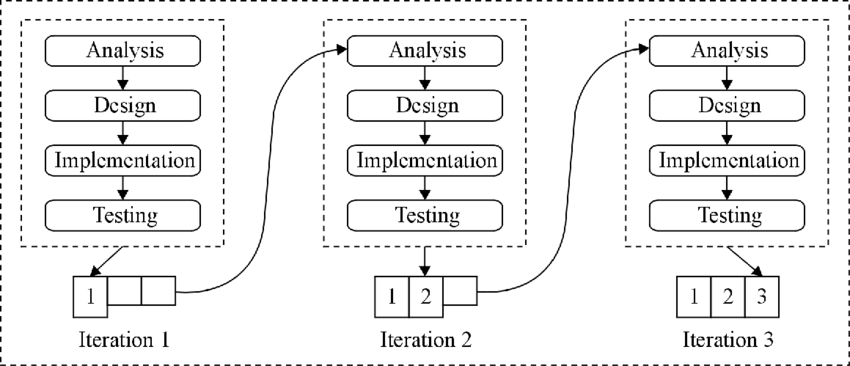
\includegraphics[width=\linewidth]{sdlc}
	\centering
	\caption{ Iterative and Incremental Approach }
	\label{fig:sdlc}
\end{figure}

The life cycle begins with the first iteration, when the team collects and evaluates the requirements that are expected from the application. The design and\\ implementation phase is to design and build both backend and client side applications. By the end of this iteration, a Minimal Viable Product (MVP) will already have been constructed. In the testing and debugging phases, the quality control methods is applied to both frontend and backend. If any changes in requirement are needed, then it can send feedback to the analysis phase that will mark the beginning of the new iteration. The project is expected to be completed in 3 iterations.
 
\pagebreak
\subsection{Technical Architecture}
The application is built upon the client-server web architecture, as illustrated in Figure \ref{fig:arch}.

\begin{figure}[h]
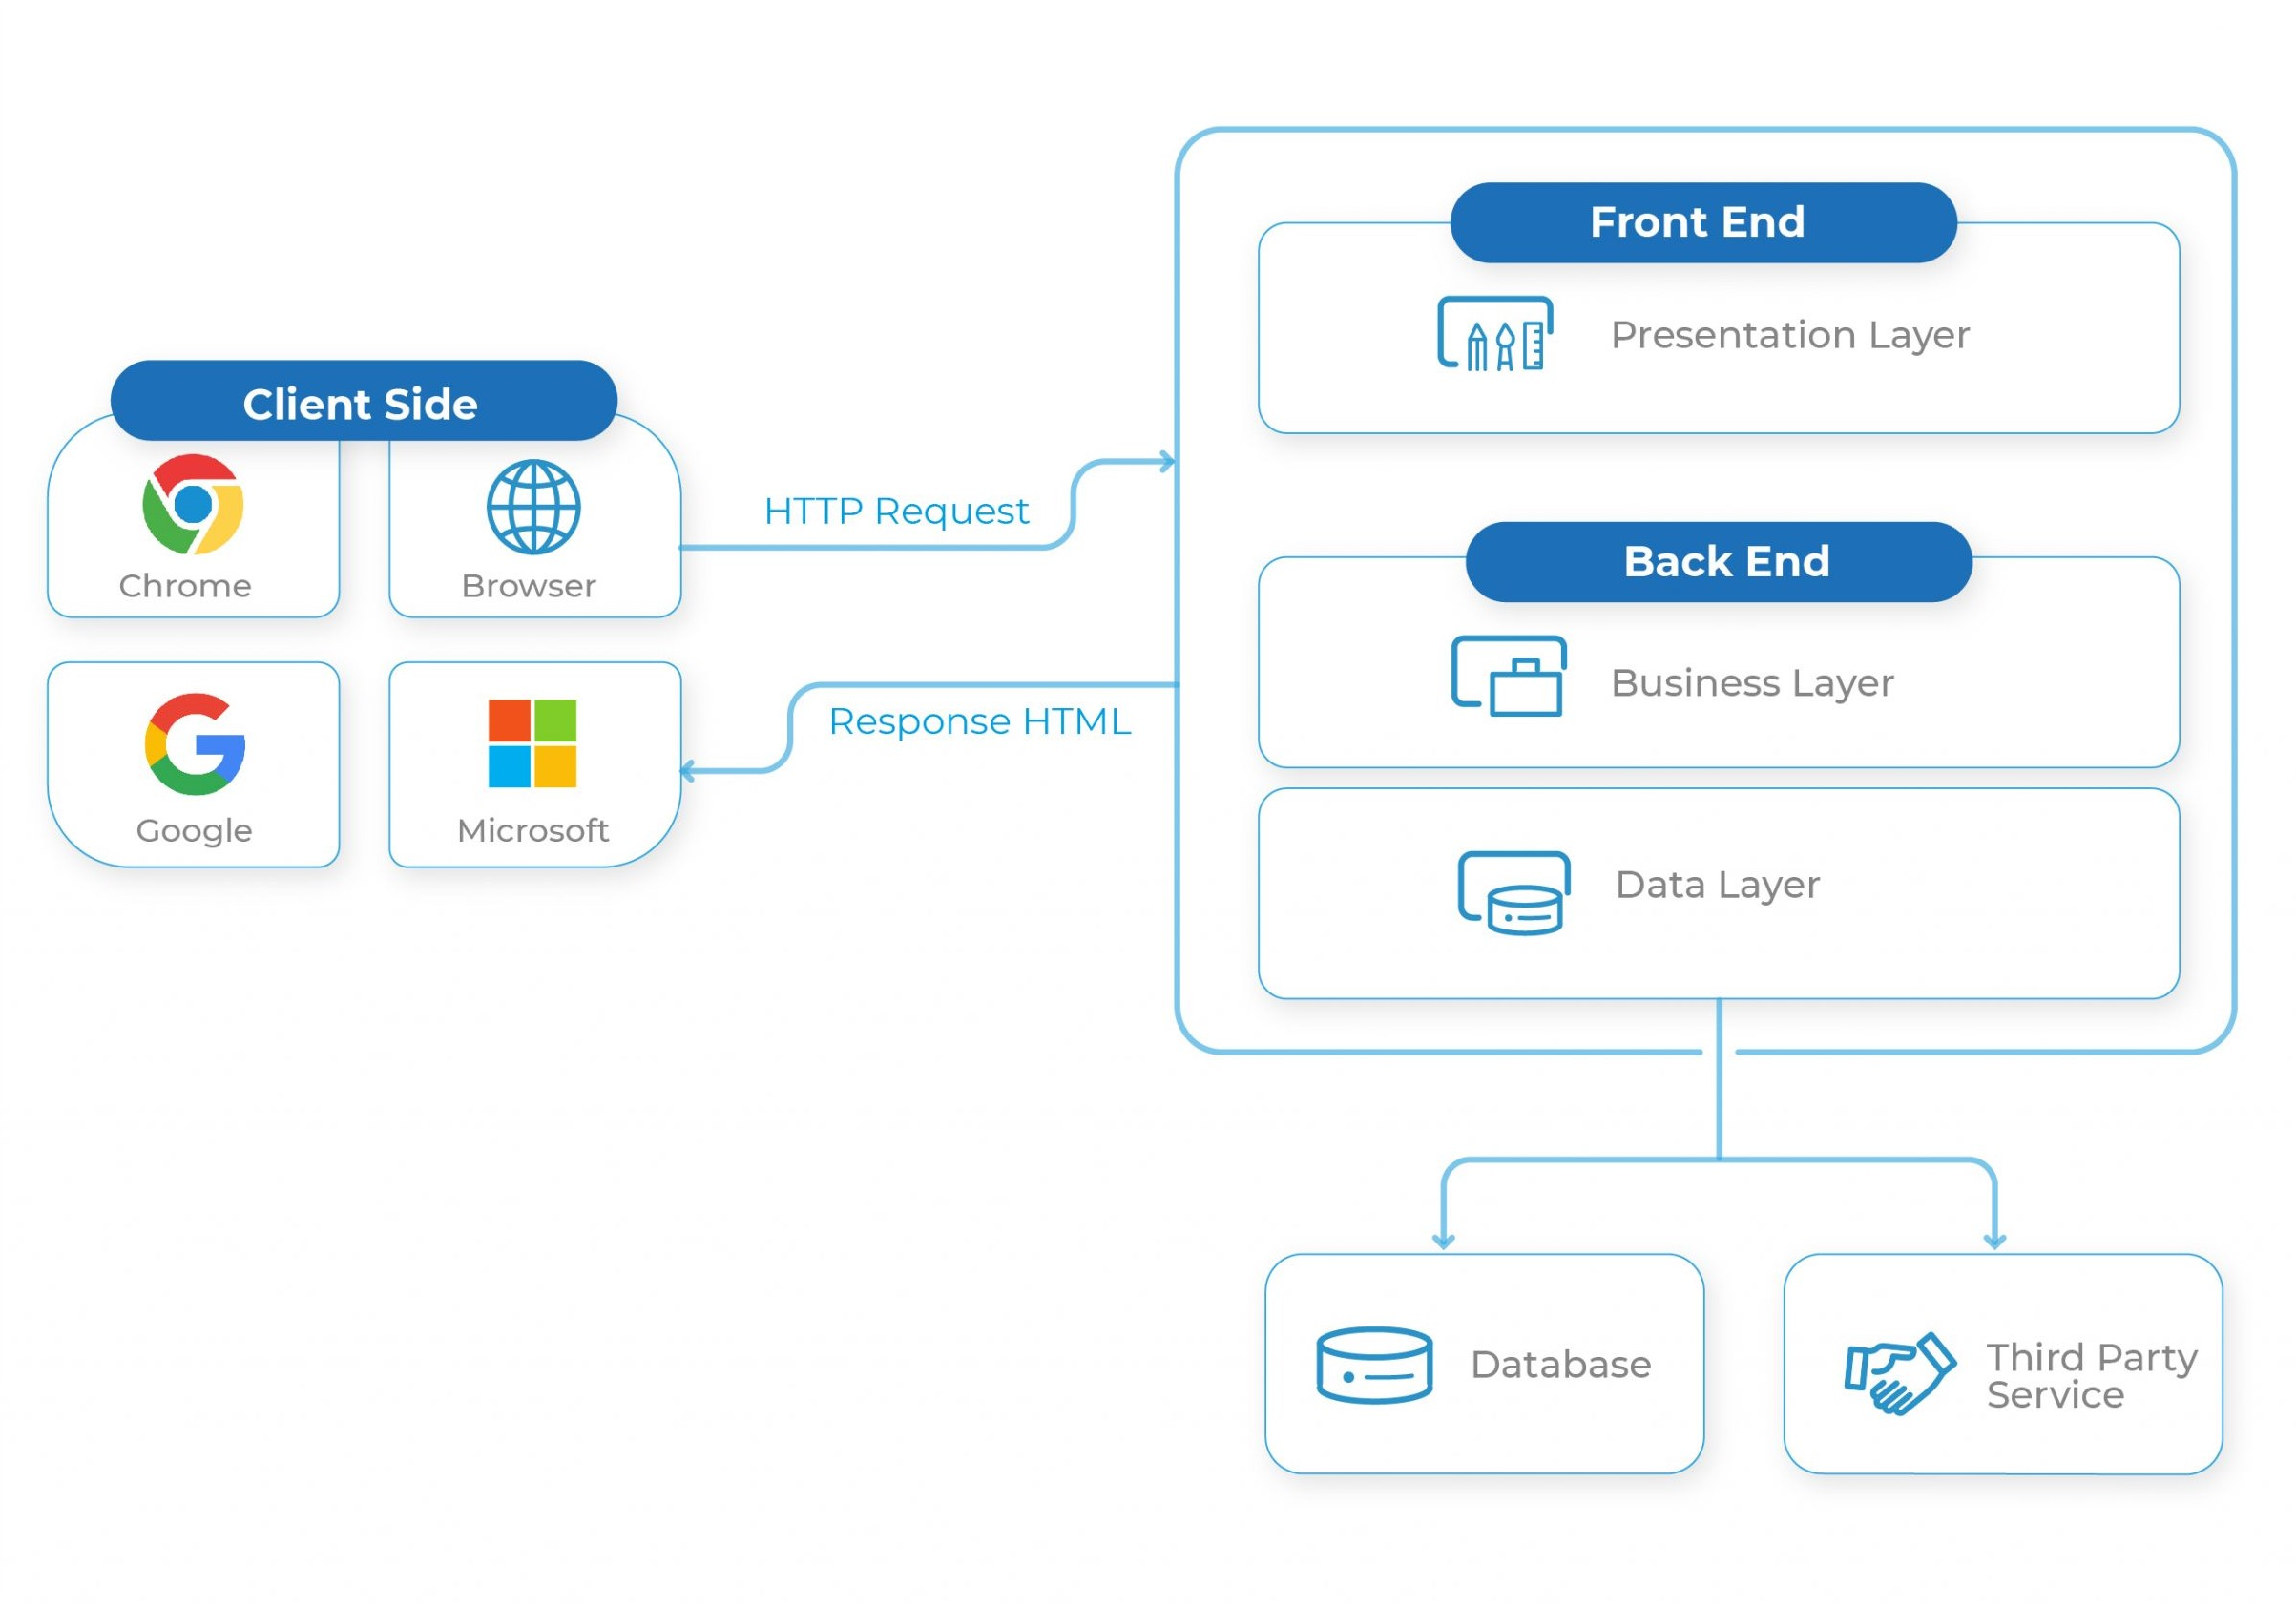
\includegraphics[width=\linewidth]{architecture}
\centering
\caption{Cilent Server web architecture}
\label{fig:arch}
\end{figure}

At the heart of the architecture lies the RESTful web service which communicates directly with the central database where all the data is stored. The client application  do not access the database directly, but via the API service. The clients send HTTP requests like GET, POST, PUT and DELETE while the API service processes those requests and return the data in JSON format. 

\pagebreak
\subsection{Used Technologies and Tools}
Table \ref{table:tech} consists of the major technologies that are used during development and deployment of the application.

\renewcommand{\arraystretch}{1.5}
\begin{table}[H]
\
\begin{tabular}{|l|l|}
\hline
\rowcolor[HTML]{C0C0C0} 
\textbf{Subject}    & \textbf{Used Technology}    \\ \hline
Database            & MongoDB                       \\ \hline
REST API Service    & Express REST Framework         \\ \hline
Frontend            & HTML, CSS, ReactJs                        \\ \hline
Backend             & NodeJs, ExpressJs             \\ \hline
Admin Web Interface & ReactJs              \\ \hline
%Deployment Platform & Amazon Web Services (AWS)      \\ \hline
Documentation & LaTeX \\ \hline
\end{tabular}
\caption{Used tools and technologies}
\label{table:tech}
\end{table}



% USE CASE AND CLASS DIAGRAMS



%\subsection{Technical Architecture}
%The application will be built upon the client-server web architecture, as illustrated in Figure \ref{fig:arch}.

%USE CASE DIGRAM
\pagebreak
\subsection*{Use Case Diagram}
A use case diagram is a way to summarize details of a system and the users within that system. It is generally shown 
as a graphic depiction of interactions among different elements in a system.
\begin{figure}[H]
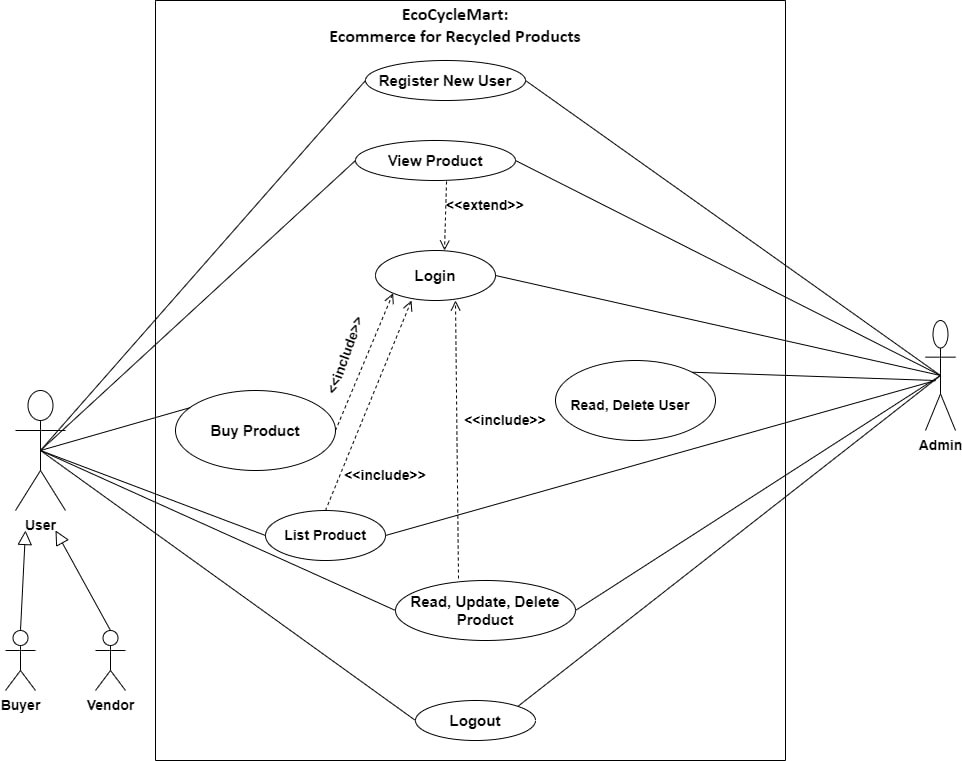
\includegraphics[width=\linewidth ]{use_case_diagram}
\centering
\caption{Use Case Diagram}
\label{fig:use_case_diagram}
\end{figure}

%CLASS DIAGRAM
\pagebreak
\section*{Class Diagaram}

A class diagram is a type of static structure diagram in the Unified Modeling Language (UML) that describes the structure of a system by showing its classes, attributes, operations, and the relationships among objects.
\begin{figure}[H]
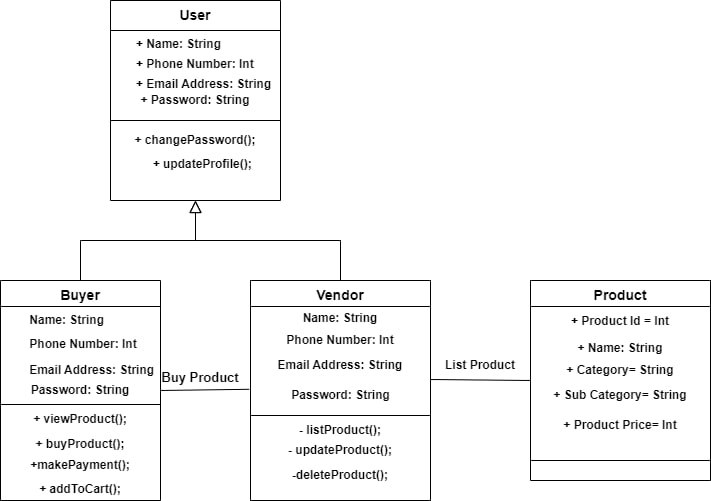
\includegraphics[width=\linewidth]{class_diagram}
\centering
\caption{Class Diagram}
\label{fig:class_diagram}
\end{figure}

\pagebreak


%khalti payment flow description



\section*{Khalti Payment Processing Flow }
\begin{itemize}
  \item \textbf{Payment Initiation}
    \begin{itemize}
      \item Customer selects Khalti.
      \item Merchant sends payment request to Khalti.
    \end{itemize}

  \item \textbf{Redirection}
    \begin{itemize}
      \item Customer redirected to Khalti's payment page.
    \end{itemize}

  \item \textbf{Authentication}
    \begin{itemize}
      \item Customer logs in or uses OTP.
      \item Khalti verifies identity and balance.
    \end{itemize}

  \item \textbf{Payment Authorization}
    \begin{itemize}
      \item Customer confirms payment.
      \item Khalti processes payment and debits wallet.
    \end{itemize}

  \item \textbf{Notification}
    \begin{itemize}
      \item Khalti sends confirmation to customer and merchant.
      \item Customer redirected back to merchant's site.
    \end{itemize}

  \item \textbf{Transaction Completion}
    \begin{itemize}
      \item Merchant validates payment and completes order.
    \end{itemize}

  \item \textbf{Settlement}
    \begin{itemize}
      \item Khalti settles payments with merchant.
    \end{itemize}
\end{itemize}
%khalti payment flow diagram
%Khalti payment diagram


\begin{figure}[H]
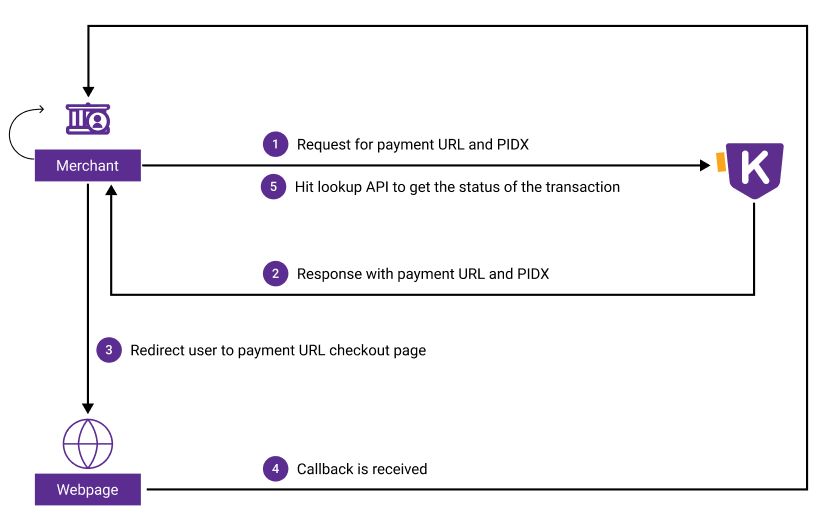
\includegraphics[width=\linewidth ]{khalti_payment_diagram}
\centering
\caption{Khalti payment flow Diagram}
\label{fig:khalti_payment_diagram}
\end{figure}

\break

% Work Details

\section{Work Details }
  \subsection{ On Backend }
   \begin{itemize}
     \item \textbf{System Requirements Gathering and Analysis }
      \begin{itemize}
      
       \item{Conducted meeting with supervisor to gather requirements.}
       \item{Analyzed the gathered requirements to identify key functionalities.}
       \item{Created a detailed system requirement specification.}
       
       \end{itemize}
       
        \item \textbf{Database Design and Implementation}
      \begin{itemize}
         \item{Designed the database schema for user, product, order, payment.}
         \item{Implemented the database using Object Relational Mapper named mongoose.}
         

       \end{itemize} 
     \item \textbf{User Module}
       \begin{itemize}
          \item{Developed APIs allowing users (Admin, Buyer and Seller) to create and manage accounts.}
          \item{Implemented user authentication functionality.}
       \end{itemize}
       
    \item \textbf{Product, Cart Module, Order Module}
       \begin{itemize}
           \item{Implemented APIs for CRUD operation.}
           \item{Implemented API features such as searching, filtering and pagination.}
           
       \end{itemize}
     
   \end{itemize}
  
\break
 \subsection{On Frontend}
  \begin{itemize}
      \item \textbf{Admin Module}
         \begin{itemize}
            \item{Interface for overview of analytical information such as total revenue, growth etc. through visualization.}
            \item{Interface to manage products, users, orders, reviews, payments.}
          
         \end{itemize}
     \item \textbf{User Module}
         \begin{itemize}
             \item{Developed Pages related to Authentication (Signin, Signup).}
             \item{Profiling and Account related pages (Update profile, Change password).}
         \end{itemize}
     \item \textbf{Product, Order, Cart and  Review Module}
        \begin{itemize}
           \item{Developed Create, Update and Detail page.}
        \end{itemize}
    \item \textbf{Cart, Checkout and Payment}
       \item \textbf{Rating, Reviews and Billing, Google Authentication.}
       \begin{itemize}
          \item{Developed interface for checkout such as adding products to cart.}
          \item{Developed interface for displaying summary of order.}
          \item{Implemented interface to allow users to input address information and choose payment method.} 
          \item{Developed interface for payment processing and confirmation.}
       \end{itemize}
       
   \item \textbf{Pages included}
       \begin{itemize}
             \item{Landing page with hero, recommended products and featured products sections.}
             \item{Products listing page with searching and filtering.}
             \item{Product detail page.}
       \end{itemize}
  \end{itemize}


  
     
   

\break


\subsection{On Artificial Intelligence}

%AI implementation\\


\subsection*{AI based Products Recommendation using
  Content based filtering }


Content-based filtering is a popular approach for building recommender systems that suggest new products or items to users based on the features or attributes of the items they have interacted with in the past.

%\subsection*{Key Concepts and Algorithms}


\subsection*{User Profile}

The user profile is a representation of the user's preferences, typically in the form of a feature vector. It is built based on the user's past interactions, such as purchases, ratings, or clicks. The user profile captures the user's interests and can be used to find similar items to recommend.

\subsection*{Item Profile}

The item profile is a representation of the features or attributes of a product or item. This could include characteristics like category, brand, price, description, etc. The item profile is used to find items that are similar to the ones the user has liked in the past.

\subsection*{Utility Matrix}

The utility matrix is a representation of the user-item interactions, where each entry indicates the user's preference or rating for a particular item. This matrix is used to understand the relationship between users and items.

\subsection*{Algorithms}

\subsection*{TF-IDF (Term Frequency-Inverse Document Frequency)}

TF-IDF is a common technique used to represent items (especially text-based items) in a feature vector format. It weighs the importance of terms within a document relative to a corpus of documents.

\subsubsection*{Term Frequency (TF)}

Measures how frequently a term appears in a document.

\[
\text{TF}(t,d) = \frac{\text{Number of times term } t \text{ appears in document } d}{\text{Total number of terms in document } d}
\]

\subsubsection*{Inverse Document Frequency (IDF)}

Measures the importance of a term by decreasing the weight of terms that appear frequently in many documents.

\[
\text{IDF}(t) = \log \left(\frac{\text{Total number of documents}}{\text{Number of documents containing term } t}\right)
\]

\subsubsection*{TF-IDF}

Combines TF and IDF.

\[
\text{TF-IDF}(t,d) = \text{TF}(t,d) \times \text{IDF}(t)
\]

\subsection*{Cosine Similarity}

Cosine similarity measures the cosine of the angle between two vectors, which in this context are the feature vectors of items or user profiles.

\[
\text{Cosine Similarity}(A,B) = \cos(\theta) = \frac{A \cdot B}{\|A\| \|B\|}
\]

Where:

\begin{itemize}
    \item \( A \cdot B \) is the dot product of vectors \( A \) and \( B \).
    \item \( \|A\| \) and \( \|B\| \) are the magnitudes (Euclidean norms) of vectors \( A \) and \( B \).
\end{itemize}

\subsection*{User Profile Creation}

User profiles can be created by averaging the feature vectors of the items the user has interacted with. If a user has interacted with \( n \) items with feature vectors \( I_1, I_2, \ldots, I_n \), the user profile vector \( U \) can be calculated as:

\[
U = \frac{1}{n} \sum_{i=1}^{n} I_i
\]

\subsection*{Similarity Score Calculation}

The similarity score between the user profile \( U \) and an item profile \( I \) is calculated using cosine similarity:

\[
\text{Similarity}(U, I) = \frac{U \cdot I}{\|U\| \|I\|}
\]

\subsection*{Weighted User Profile Creation}

If items have different levels of importance or ratings, the user profile can be weighted accordingly. Let \( w_i \) be the weight (e.g., rating) of item \( i \). The weighted user profile \( U_w \) is:

\[
U_w = \frac{\sum_{i=1}^{n} w_i \cdot I_i}{\sum_{i=1}^{n} w_i}
\]

\subsection*{Example}

Let's consider a simplified example of how these formulas are used in practice:

\subsection*{Item Profiles}

Assume we have two items with the following feature vectors:

\[
I_1 = [0.2, 0.4, 0.4]
\]

\[
I_2 = [0.1, 0.8, 0.1]
\]

\subsection*{User Profile}

The user has interacted with these two items equally. The user profile \( U \) is:

\[
U = \frac{1}{2} \left(I_1 + I_2\right) = \frac{1}{2} \left([0.2, 0.4, 0.4] + [0.1, 0.8, 0.1]\right) = [0.15, 0.6, 0.25]
\]

\subsection*{Similarity Calculation}

To recommend a new item with profile \( I_3 = [0.3, 0.3, 0.4] \), we calculate the cosine similarity between \( U \) and \( I_3 \):

\[
\text{Similarity}(U, I_3) = \frac{[0.15, 0.6, 0.25] \cdot [0.3, 0.3, 0.4]}{\|[0.15, 0.6, 0.25]\| \|[0.3, 0.3, 0.4]\|}
\]

\subsubsection*{Dot Product}

\[
0.15 \cdot 0.3 + 0.6 \cdot 0.3 + 0.25 \cdot 0.4 = 0.045 + 0.18 + 0.1 = 0.325
\]

\subsubsection*{Magnitudes}

\[
\|[0.15, 0.6, 0.25]\| = \sqrt{0.15^2 + 0.6^2 + 0.25^2} = \sqrt{0.0225 + 0.36 + 0.0625} = \sqrt{0.445} \approx 0.667
\]

\[
\|[0.3, 0.3, 0.4]\| = \sqrt{0.3^2 + 0.3^2 + 0.4^2} = \sqrt{0.09 + 0.09 + 0.16} = \sqrt{0.34} \approx 0.583
\]

\subsubsection*{Final Similarity Calculation}

\[
\text{Similarity}(U, I_3) = \frac{0.325}{0.667 \times 0.583} \approx \frac{0.325}{0.389} \approx 0.835
\]

The similarity score of 0.835 indicates a high degree of similarity between the user profile and item \( I_3 \), suggesting that \( I_3 \) would be a good recommendation for the user.

      

\begin{figure}[H]
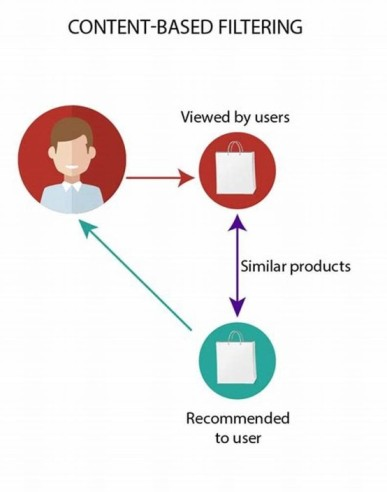
\includegraphics[width=\linewidth ]{content_based_filtering}
\centering
\caption{Content Based Filtering}
\label{fig:content_based_filtering}
\end{figure}
      






\break

%\section{Results and Discussion }

 % In this section , we present the results and discuss the findings of the completed tasks. The key 
%points for discussion include:
%\begin{itemize}
  
 %   \item{ Discussed about the user signup, admin dashboard and report format.}
  %  \item {Discussion on payment method and report revision.}
   % \item{User authentication and  profiling.}
   % \item {Rating and reviews )}
    %\item {Cart functionality, Checkout and Payment processing.}
    %\item {Product, Order and User management from admin panel.}
%\end{itemize}



%results and discussion

\break



\break 


\section{Performance Analysis and Validation Scheme}

This involves evaluating the system's functionality, performance, usability, and security through a systematic approach.

\subsection{Functional Analysis}

\begin{itemize}
  \item \textbf{Requirement Validation}: Review initial requirements documentation to verify all features and functionalities.
  \item \textbf{User Acceptance Testing}: Collaborate with users or a representative group to test the system's functionality.
\end{itemize}

\subsection{Performance Analysis}

\begin{itemize}
  \item \textbf{Stress Testing}: Apply extreme workload conditions to determine system breaking points.
  \item \textbf{Response Time Analysis}: Measure and analyze response times for various operations.
\end{itemize}

\subsection{Usability Analysis}

\begin{itemize}
  \item \textbf{User Interface Evaluation}: Assess visual design, layout, and aesthetics for usability.
  \item \textbf{User Flow Analysis}: Evaluate navigation and user flow to ensure ease of use.
\end{itemize}

\subsection{Security Analysis}

\begin{itemize}
  \item \textbf{Data Protection}: Securely store and transmit sensitive user information.
  \item \textbf{User Authentication and Authorization}: Implement robust access controls to protect user accounts.
\end{itemize}

\break
\subsection{Feasibility Analysis}

\begin{itemize}
  \item \textbf{Technical Feasibility}: Ensure required technology is available.
  \item \textbf{Economical Feasibility}: Ensure costs remain within an affordable range.
  \item \textbf{Operational Feasibility}: Ensure the project can be effectively used by its target users.
\end{itemize}

\subsection{Validation Scheme}

\begin{itemize}
  \item \textbf{Test Plan Creation}: Develop a comprehensive plan outlining testing methodologies and tools.
  \item \textbf{Test Execution}: Execute defined test cases, record results, and address any issues.
\end{itemize}



\break


      



\break
%\section{ Deliverable}
%The following are the major deliverables that are produced at the end of this project.

%\subsection{RESTful API service}
%There are running instances of RESTful API service developed and deployed at the end of the project. This API is responsible for communicating between the client applications and the central database server.

%\subsection{Frontend and Admin Dashboard}
%The application is developed integrating all the features proposed earlier. The sellers are able to use the application to list their products which are visible to the buyers. An interactive chat box is integrated with the application that will allow the users to make queries. The application will also be integrated with google authentication, payment processing, AI based recommendation system. The application is featured with order tracking abilities. 

%\subsection{Miscallaneous}
 %  \begin{itemize}
  %     \item{ A comprehensive plan outlining the project objectives, scope, timeline, resources and 
%responsibility of the team members.}
   %    \item{A final report summarizing the project’s outcomes, lessons, learned and 
%recommendations for future improvement.}
 %  \end{itemize}


%\pagebreak
%\section{Project Task and Time Schedule}
%The working time period for the project is less than three months. The %project is completed by the end of the spring semester as per the %requirements of the university. The major task division among the team %members is mentioned in Table \ref{table:taskdiv}.

%\begin{table}[h!]
%\begin{tabular}{|l|l|}
%\hline
%\rowcolor[HTML]{C0C0C0} 

%\textbf{Team Member} & \textbf{Assigned Tasks}                                                                                                                     \\ \hline
%Rishikesh Sharma       & \begin{tabular}[c]{@{}l@{}} Project Management \\ %AI Implementation \end{tabular} \\ \hline
%Hansika Jha   & \begin{tabular}[c]{@{}l@{}}Frontend Design \\ Project Documentation\end{tabular}                                           \\ \hline
%Sandip Shah   & \begin{tabular}[c]{@{}l@{}}Frontend Development\\ Project Documentation\end{tabular}                                           \\ \hline
%Kishore Budhathoki  & \begin{tabular}[c]{@{}l@{}}Backend Development\\ Data Management\\
 %\end{tabular}                                           \\ \hline
%\end{tabular}
%\caption{Division of tasks among project team members}
%\label{table:taskdiv}

%\end{table}

%\pagebreak
%\break
% The time schedule for the development of the project is illustrated in  figure \ref{figure:gantt_chart}.


% \begin{figure}[h!]
% 	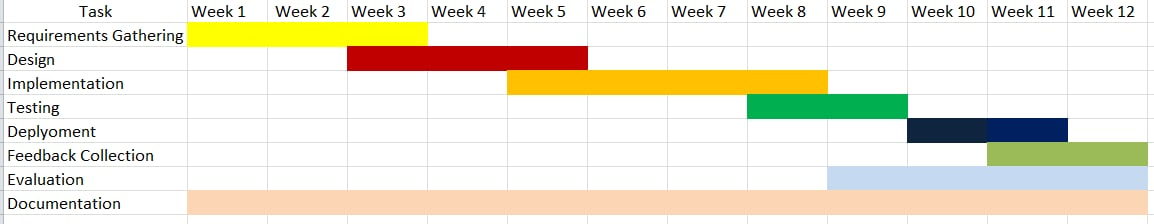
\includegraphics[width=\linewidth]{gantt_chart}
% 	\centering
% \caption{Gantt Chart}
% 	\label{figure:gantt_chart}
% \end{figure}


%\pagebreak

%conclusion



\section{Conclusion}
The EcoCycleMart web app is developed using Visual studio code. We have collected all the important knowledge and useful skills for developing an ecommerce platform. By a helpful guidance of the supervisor and with team work, we are determine to make this project a success.


\pagebreak


\section{Further Works}

\begin{itemize}
   \item {Native Applications such as mobile and desktop will be built.}
   \item {Integrate other payment service gateway.}
   \item {Build dataset for localized recycle based products }
   
\end{itemize}
\pagebreak


%\break
\section{References}
\bibliography{references}
\bibliographystyle{IEEEtran}
@misc{GeoTrust,
title={Creating an E-Commerce web site},
place={california},
url={https://www.geotrust.com/resources/guides/creating-ecommerce-website.pdf},
year={2010}
},

@misc{journal,
title={The Role of E-Commerce in Sustainable Supply Chain Management},
publisher={Xiutian Shi et al},
year={2019},
}

@misc{similarapps,
title={Jamarko},
url={https://jamarko.com.np/},
journal={MakeUseOf},
description={
Online website for selling recycled paper material goods in Nepal.
},
}

@article{cirlulareconomy,
  title={Circular Economy Principles},
  author={Warner, Jon S and Johnston, Roger G},
  institution={Ellen MacArthur Foundation},
  description={Provides Insights and resources on circular economy principles},

}

@article{reactjs,
title={A Comprehensive Guide to React.js},
url={https://flaviocopes.com/react/},
author={Flavio Copes},
year={2021}
}


@misc{nodejstutorial,
title={Node.js Tutorial for Beginners  Learn Node in 1 Hour},
url={https://www.youtube.com/watch?v=TlB\_eWDSMt4},
year={2018}
}

@misc{recommendersystems,
title={Recommender Systems: An Introduction},
author={ Dietmar Jannach, Markus Zanker, Alexander Felfernig and Gerhard Friedrich }

@misc{lightfm,
title={LightFM},
url={https://github.com/lyst/lightfm},
description={A Python implementation of a number of popular recommendation algorithms for both implicit and explicit feedback.}
}

}

\break

%appendix

\section{Appendix}


\subsection*{ Admin and User Interface}
%admin and user interface

%landing page
\begin{figure}[H]
\captionsetup{list=false}
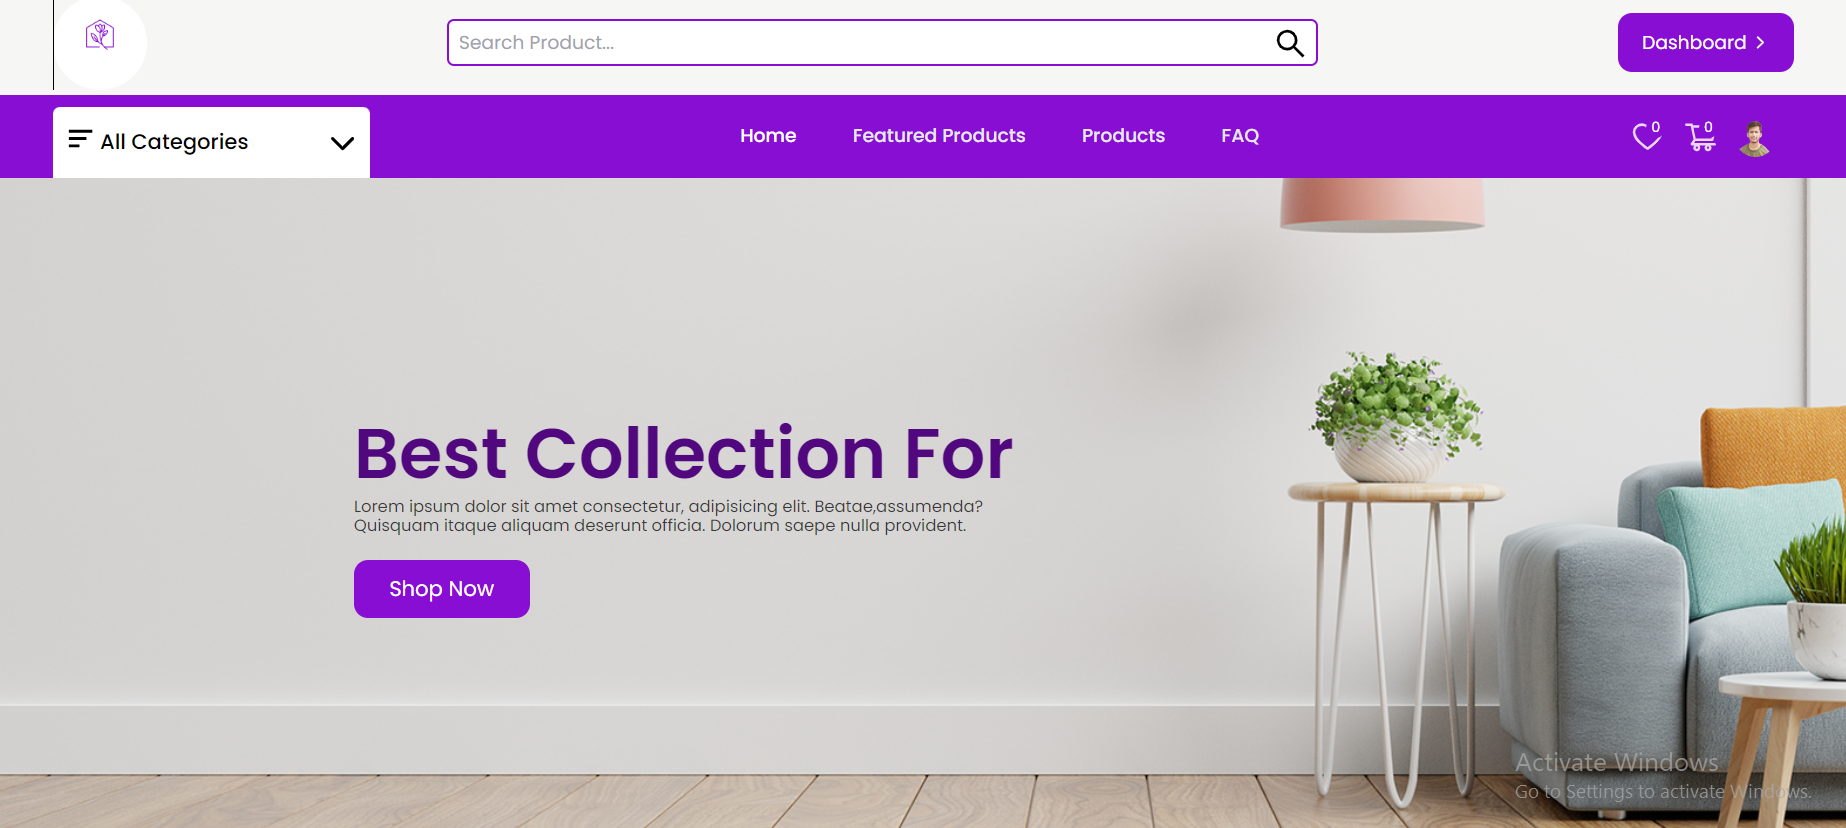
\includegraphics[width=\linewidth ]{landing_page}
\centering
\caption{Landing Page}
%\label{fig:landing_page}
\end{figure}

%admin dashboard main
\begin{figure}[H]
\captionsetup{list=false}
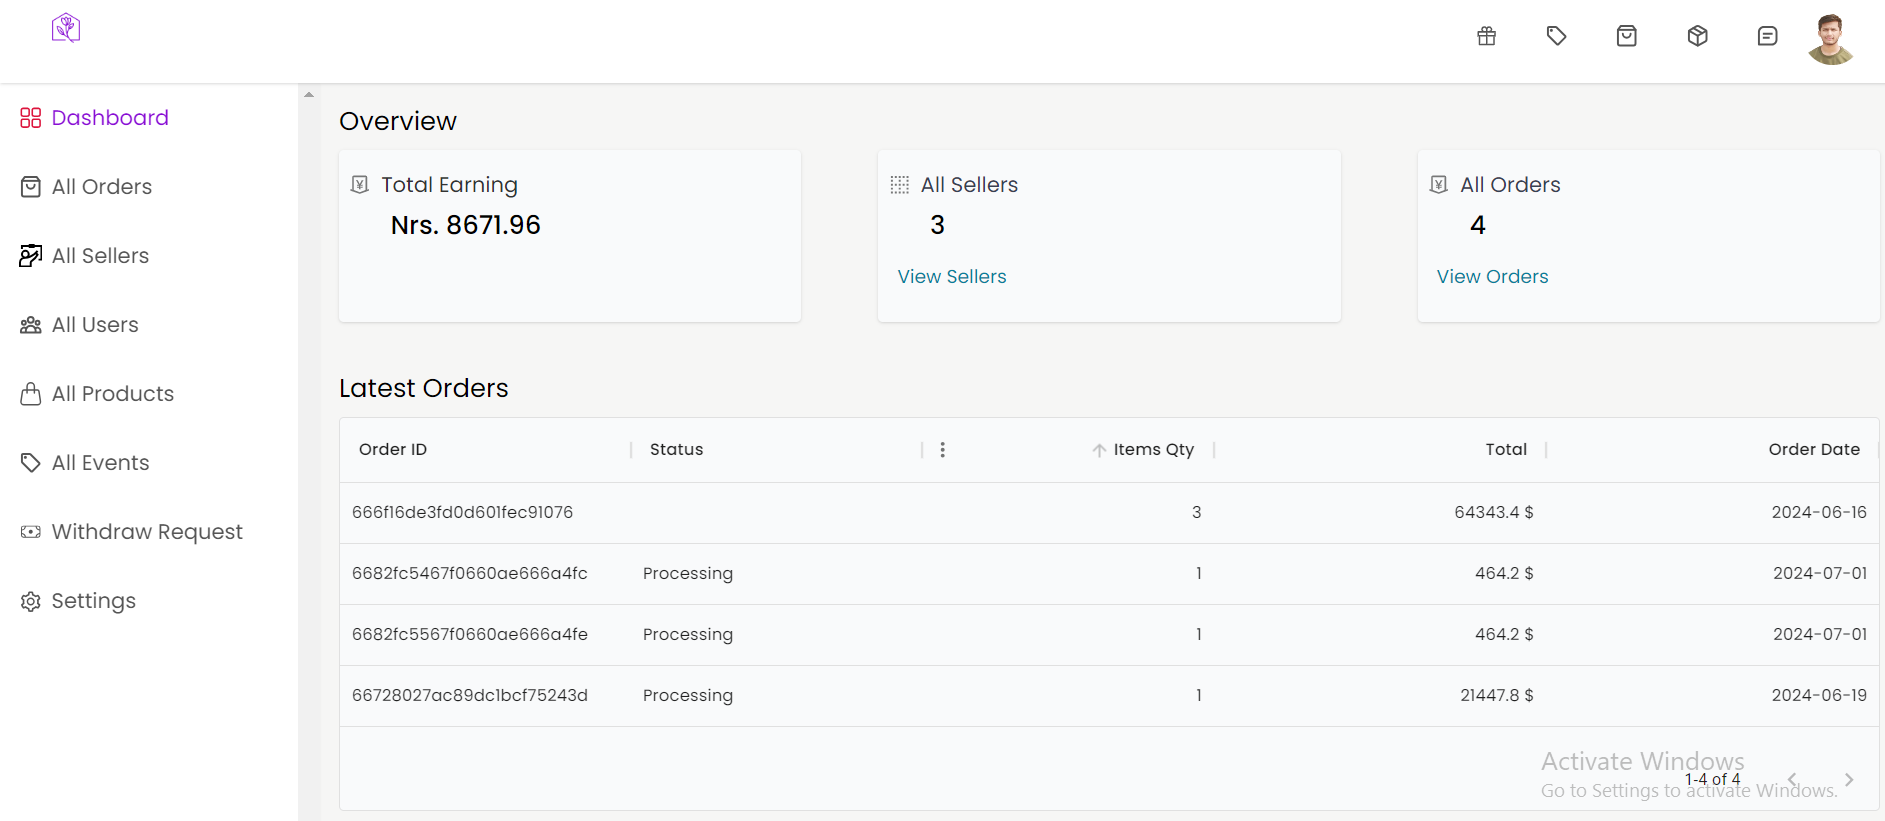
\includegraphics[width=\linewidth ]{admin_main}
\centering
\caption{Admin Overview Page}
\label{fig:admin_main}
\end{figure}



\subsection*{ Checkout and Payment Processing}
%Checkout UI
\begin{figure}[!h]
\captionsetup{list=false}
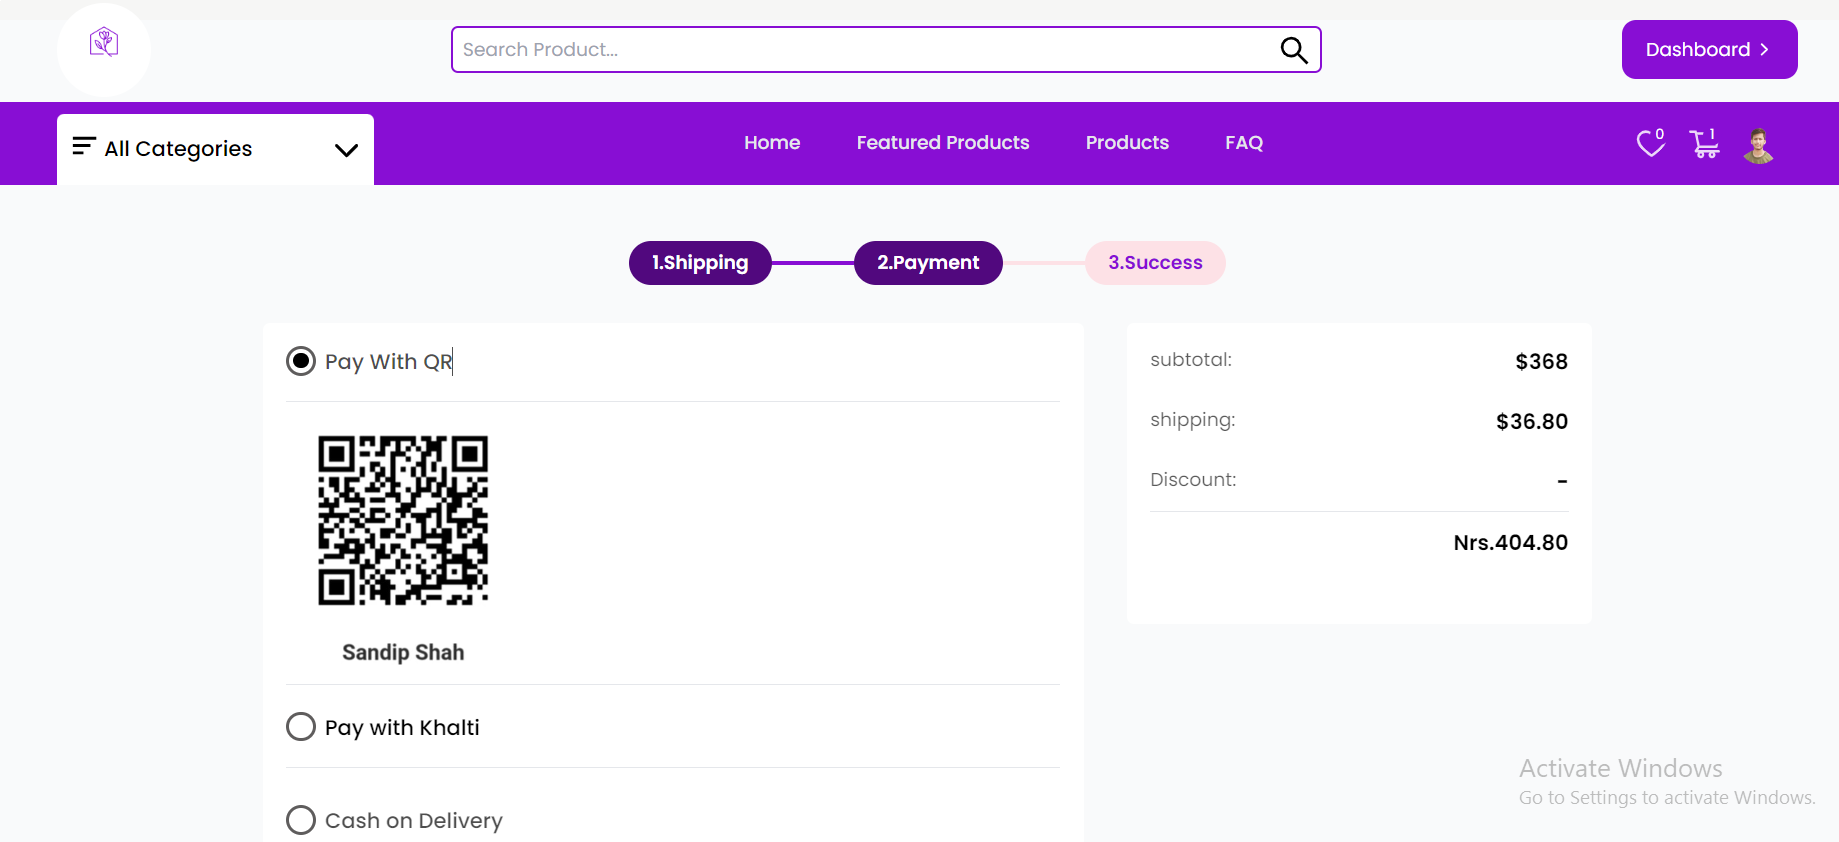
\includegraphics[width=\linewidth ]{checkout_ui}
\centering
\caption{Checkout User Interface}
\label{fig:checkout_ui}
\end{figure}


%Khalti payment widget
\begin{figure}[!h]
 \captionsetup{list=false}
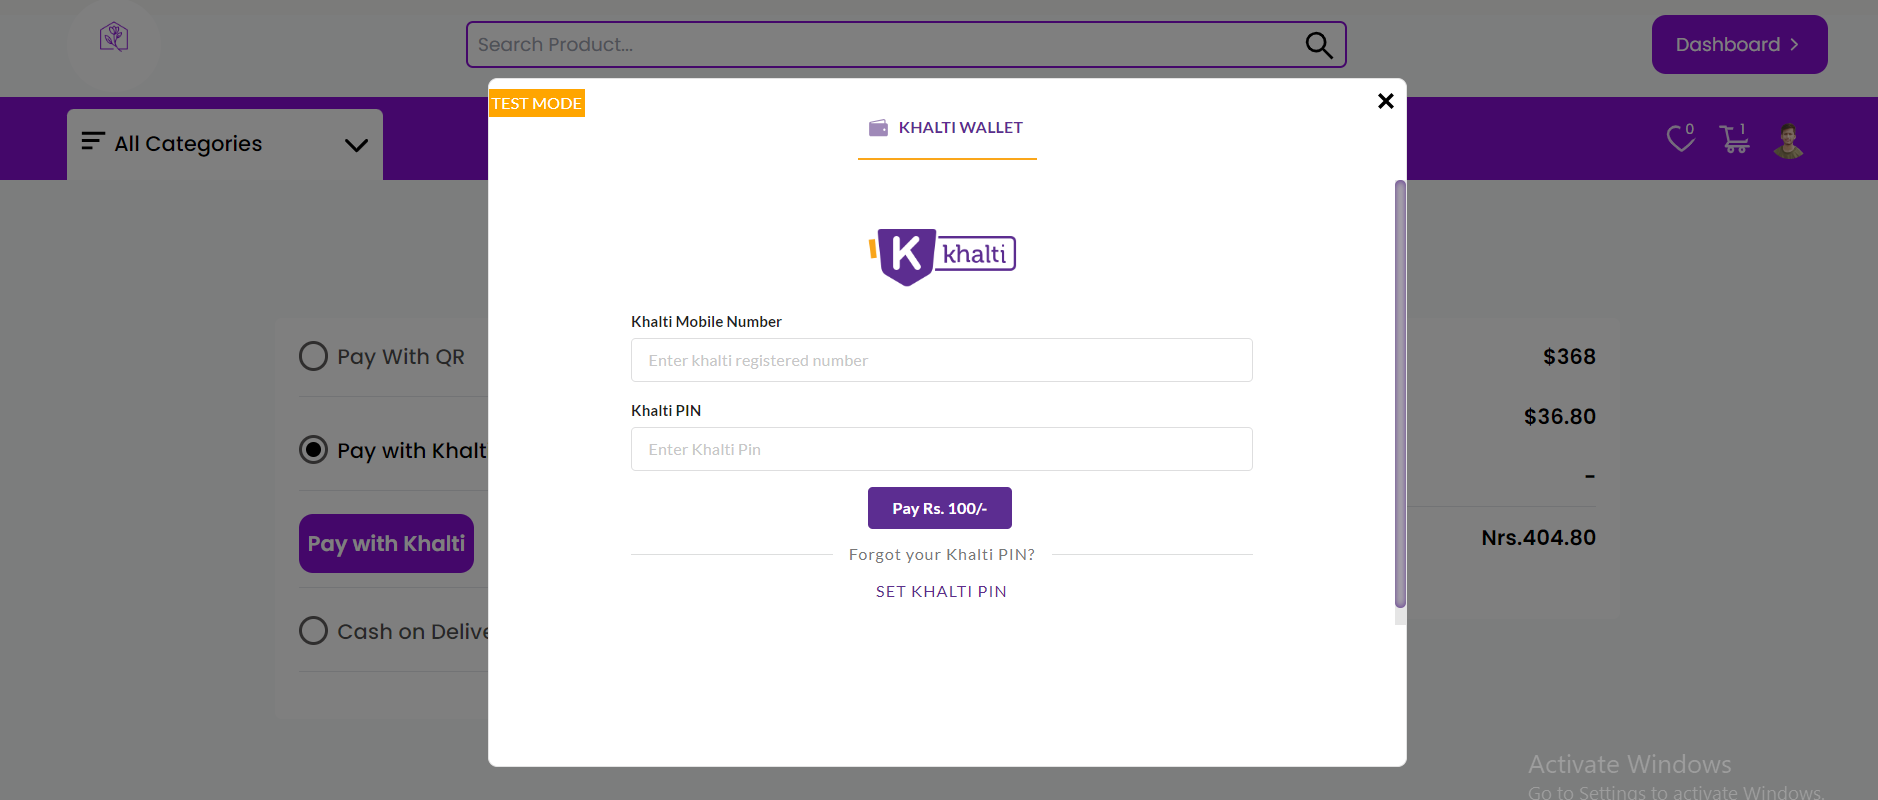
\includegraphics[width=\linewidth ]{khalti_widget}
\centering
\caption{Payment Using Khalti}
\label{fig:khalti_widget}
\end{figure}


\subsection*{ Profiling}
%Profiling
\begin{figure}[!h]
\captionsetup{list=false}
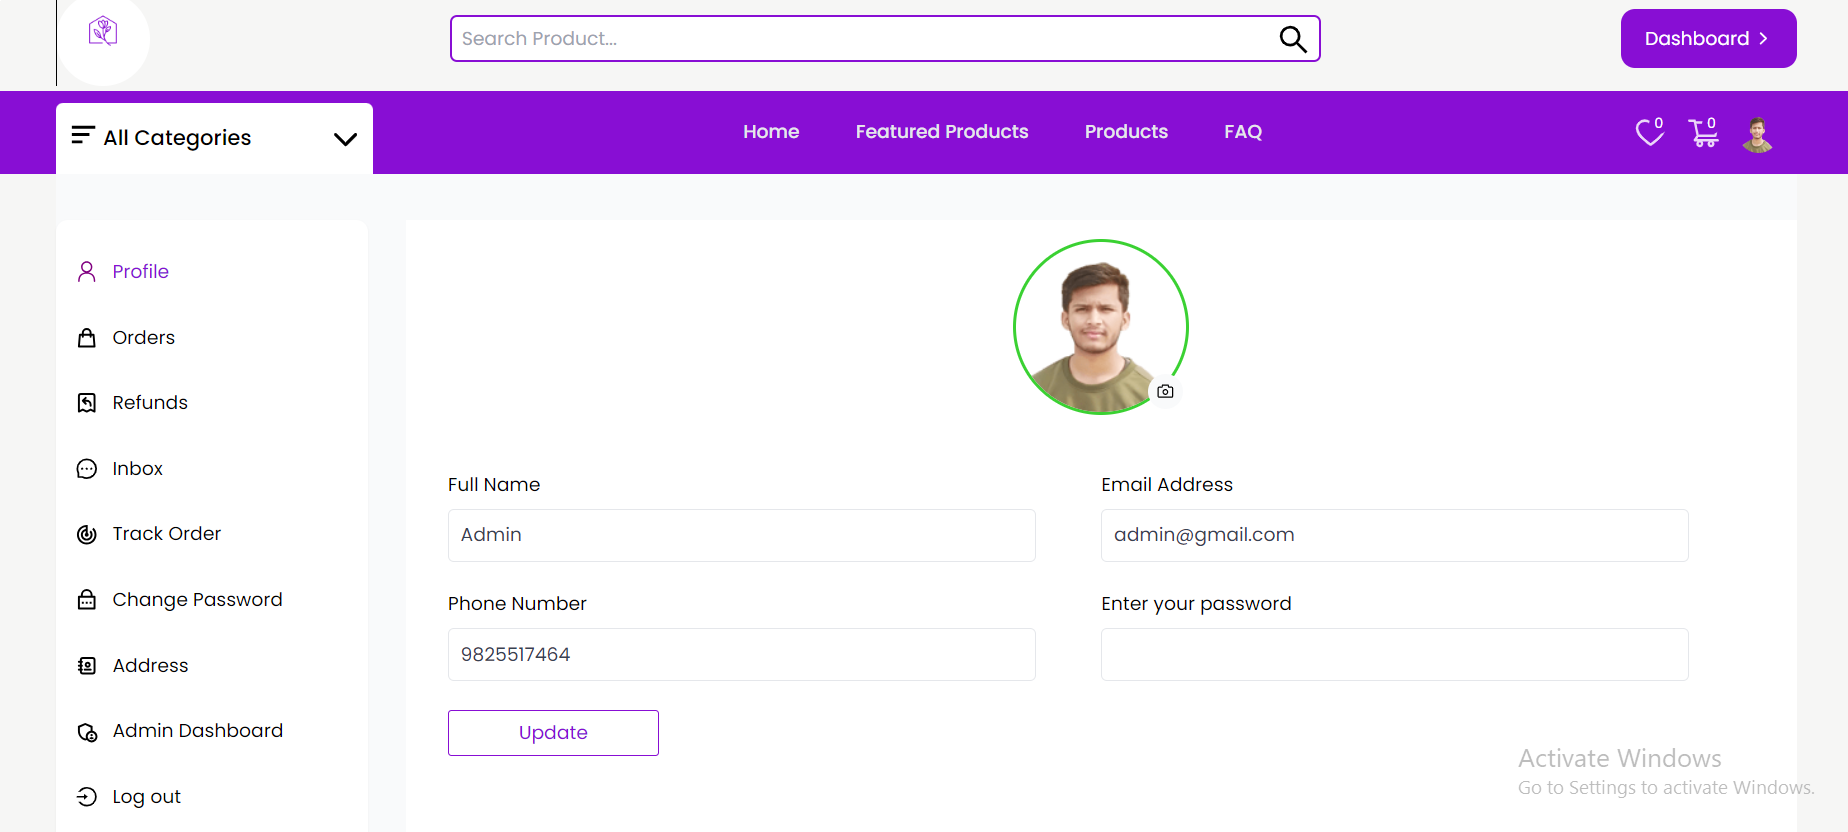
\includegraphics[width=\linewidth ]{profile_page}
\centering
\caption{Profile Page}
\label{fig:profile_page}
\end{figure}


\break
\pagebreak
\newpage
\subsection*{ Exploratory Data Analysis}
%Distribution of Interaction of Data per Item and Distribution of Interaction of Data per User
\begin{figure}[!h]
\captionsetup{list=false}
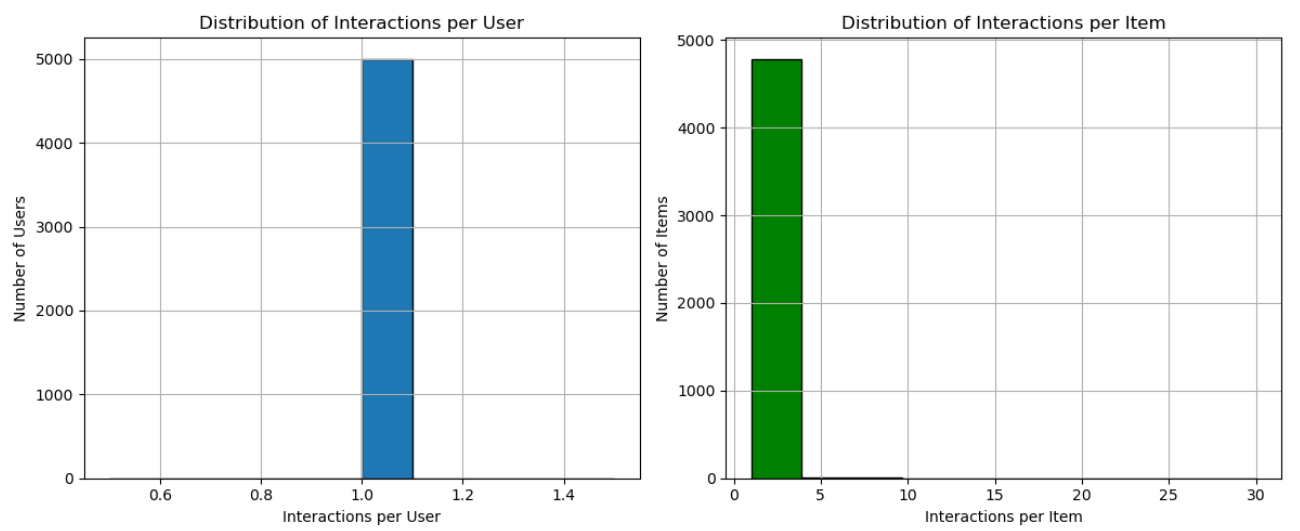
\includegraphics[width=\linewidth ]{dipi_dipu}
\centering
\caption{Distribution of Interaction of Data per Item and Distribution of Interaction of Data per User}
\label{fig:dipi_dipu}
\end{figure}

%Most popular items
\begin{figure}[!h]
\captionsetup{list=false}
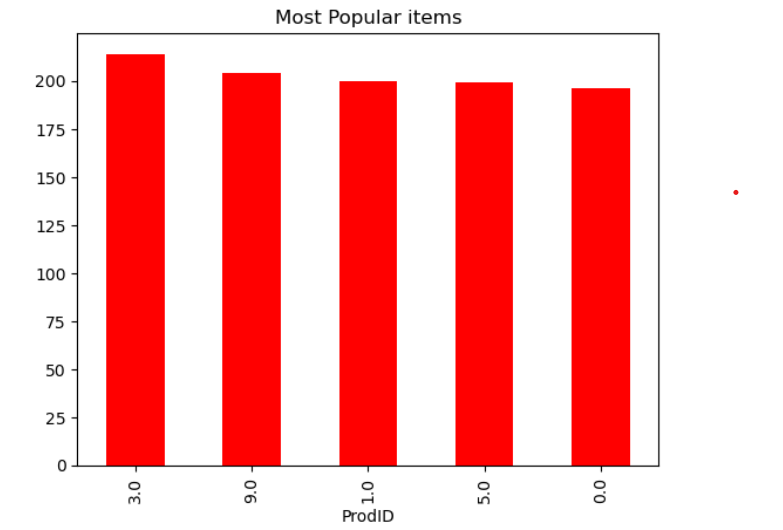
\includegraphics[width=\linewidth ]{most_popular_items}
\centering
\caption{Most Popular Items}
\label{fig:most_popular_items}
\end{figure}


%Most rated counts
\begin{figure}[!h]
\captionsetup{list=false}
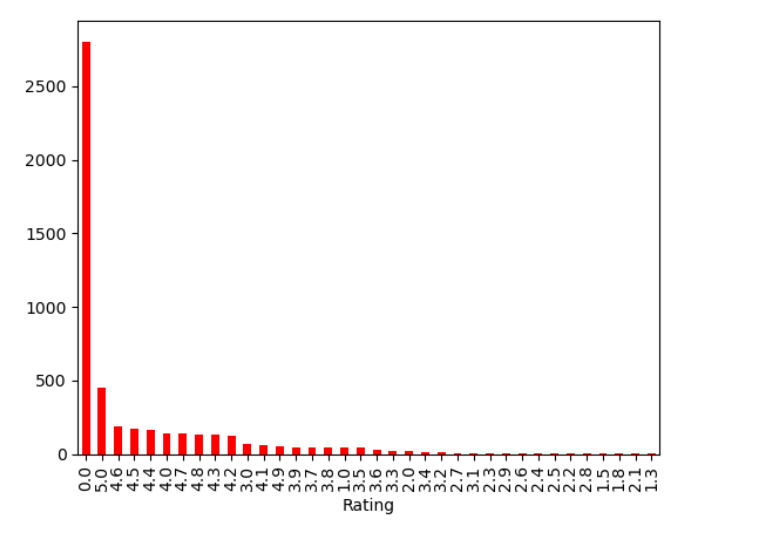
\includegraphics[width=\linewidth ]{most_rated_counts}
\centering
\caption{Most Rated Counts}
\label{fig:most_rated_counts}
\end{figure}

\end{document}

\break



